\documentclass{beamer}
\usetheme[pageofpages=of,% String used between the current page and the
                         % total page count.
          bullet=circle,% Use circles instead of squares for bullets.
          titleline=true,% Show a line below the frame title.
          alternativetitlepage=true,% Use the fancy title page.
       %   titlepagelogo=logo-polito,% Logo for the first page.
       %   watermark=watermark-polito,% Watermark used in every page.
       %   watermarkheight=100px,% Height of the watermark.
       %   watermarkheightmult=4,% The watermark image is 4 times bigger
                                % than watermarkheight.
          ]{Torino}

\setbeamertemplate{footline}{
  \begin{beamercolorbox}[wd=\paperwidth,ht=1ex,dp=1ex]{footline}
    \vspace{5pt} \hspace{1em} \insertframenumber/\inserttotalframenumber
  \end{beamercolorbox}
}

\author{Brendon J. Brewer}
\title{STATS 331 -- Introduction to Bayesian Statistics}
\institute{The University of Auckland}
\date{}


\linespread{1.3}
\usepackage{minted}
\usepackage[utf8]{inputenc}
\usepackage{dsfont}


\begin{document}

\frame{\titlepage}

\begin{frame}
\centering

\includegraphics[width=0.8\textwidth]{images/dilbert.jpg}

\end{frame}



\begin{frame}
\centering
\large
Bayesian Linear Regression

\end{frame}


\begin{frame}
\frametitle{Models}
\begin{itemize}
\item We have seen most of the fundamental principles that we will need
throughtout the course.\pause
\item From now on, most of what we will study are particular `models'
for common data analysis situations.\pause
\item We will start with simple linear regression.
\end{itemize}

\end{frame}



\begin{frame}
\frametitle{Road Sign Data}
\centering
\includegraphics[width=0.8\textwidth]{images/road_data.pdf}
\end{frame}


\begin{frame}[fragile]
\frametitle{Classical Least Squares Regression in R}
\tiny
\begin{minted}{r}
> data = read.table("road.txt")
> result = lm(data[, 2] ~ data[, 1])
> summary(result)

Call:
lm(formula = data[, 2] ~ data[, 1])

Residuals:
    Min      1Q  Median      3Q     Max 
-78.231 -41.710   7.646  33.552 108.831 

Coefficients:
            Estimate Std. Error t value Pr(>|t|)    
(Intercept) 576.6819    23.4709  24.570  < 2e-16 ***
data[, 1]    -3.0068     0.4243  -7.086 1.04e-07 ***
---
Signif. codes:  0 ‘***’ 0.001 ‘**’ 0.01 ‘*’ 0.05 ‘.’ 0.1 ‘ ’ 1

Residual standard error: 49.76 on 28 degrees of freedom
Multiple R-squared:  0.642,	Adjusted R-squared:  0.6292 
F-statistic: 50.21 on 1 and 28 DF,  p-value: 1.041e-07
\end{minted}

\end{frame}

\begin{frame}[fragile]
\frametitle{Classical Least Squares Regression in R}
\begin{minted}{r}
plot(data[, 1], data[, 2])
abline(result)
\end{minted}

\end{frame}

\begin{frame}
\frametitle{Classical Least Squares Regression in R}
\centering
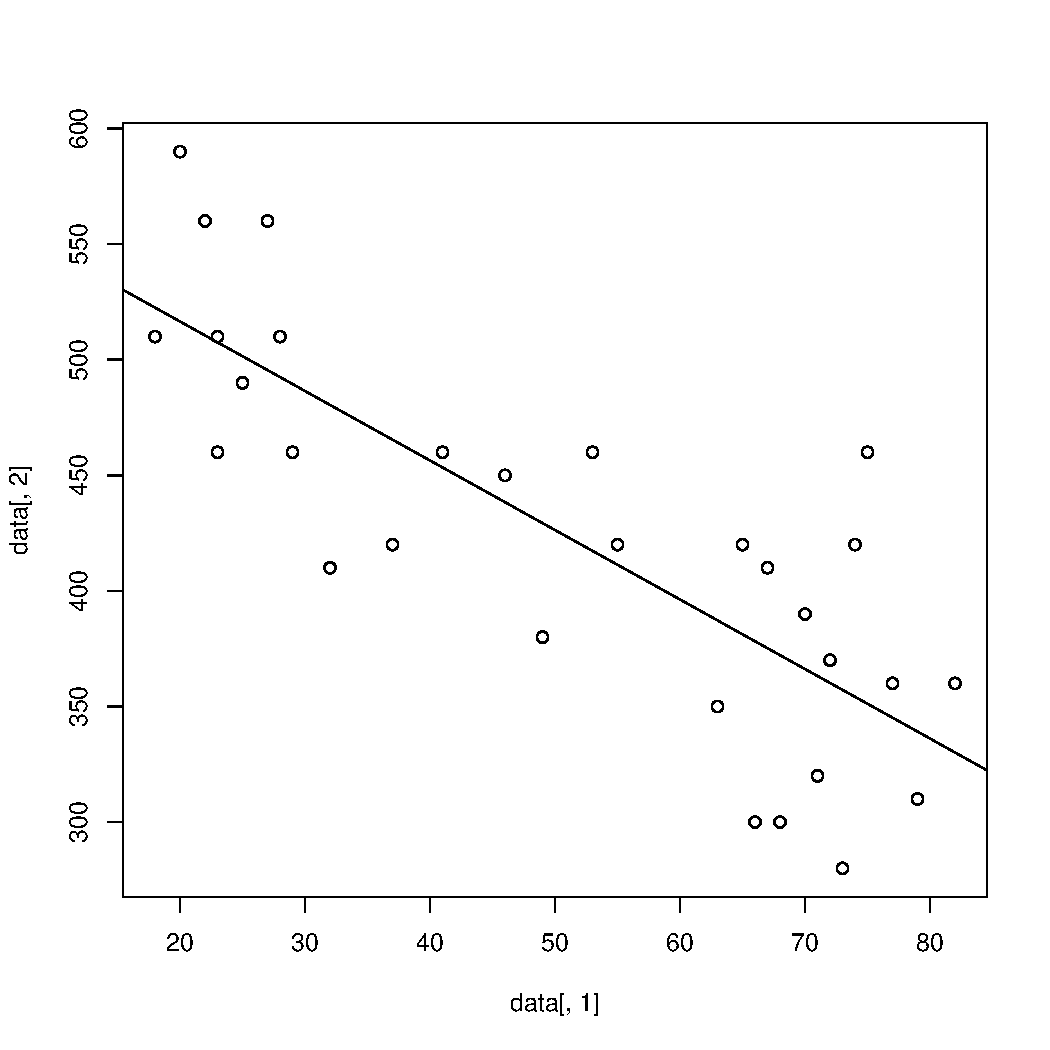
\includegraphics[width=0.6\textwidth]{images/road_lm.pdf}
\end{frame}

\end{document}

